\documentclass[xcolor=pdftex,dvipsnames]{beamer}

\usepackage{amsmath}
\usepackage{amssymb}
\usepackage{comment}
\usepackage{textcomp}

\title{Microeconomic Theory --- ECON 323 503 \\ Chapter 5: Consumer
  Welfare and Policy Analysis}
\author{Vikram Manjunath}
\institute{Texas A\&M University}
\setbeamertemplate{navigation symbols}{}
\setbeamertemplate{footline}{}
\usefonttheme{serif}
\begin{document}

\maketitle

\begin{frame}
\frametitle{Outline}
\begin{enumerate}[<+->]
\item Consumer welfare: how do we measure the effect of a price change
  on a consumer?
\item Expenditure function and consumer welfare: how much money would
  we need to give a consumer to compensate him for a price change?
\item Market consumer surplus: we can add up the individual effects to
  get the effect on the entire market.
\item Effects of government policies on consumer welfare: consumer
  welfare lets us measure the effects of various policies.
\end{enumerate}
\end{frame}

\begin{frame}
\frametitle{Consumer welfare}
If you know the utility function: easy to measure the effect of price
change.
\bigskip

\uncover<2->{
Just look at utility before and after.
}
\bigskip
\uncover<3->{

Two problems:}

\bigskip
\uncover<4->{
1. We don't know utility functions.
}
\bigskip

\uncover<5->{
2. What does it mean if you get utility 1,000 from a bundle and I get
900 from the same bundle? Nothing.

}
\end{frame}




\begin{frame}
\frametitle{Consumer welfare}
Measure consumer welfare in \emph{willingness to pay} (\$).

\bigskip
\uncover<2->{We can understand what it means if you're willing to give up \$1,000
for a bundle that I'm only willing to give up \$900 for. 
}

\uncover<3->{\bigskip
In this sense, it makes sense that you value it more than I do.}
\end{frame}




\begin{frame}
\frametitle{Consumer welfare}
\emph{Consumer surplus}: benefit from consuming the good beyond what
it cost.

\bigskip
\uncover<2->{ If you buy  product for \$1,000 and that's exactly what it's worth to
you: your welfare is 0.}

\bigskip
\uncover<3->{ If you buy  product for \$1,000 but it's worth \$2,000 to you: your welfare is \$1,000.}


\end{frame}




\begin{frame}
\frametitle{Willingness to pay}
\emph{Inverse demand function:}
\[
p=p(Q).
\]
You can use the demand function $(Q=D(p))$ to get this.

\bigskip
\uncover<2->{ Inverse demand function tells us the \emph{marginal willingness to
  pay} for a good.}

\bigskip
\uncover<3->{ This is the \emph{marginal value} that you assign to getting one more
unit of the good.}


\end{frame}




\begin{frame}
\frametitle{Willingness to pay}
\begin{center}
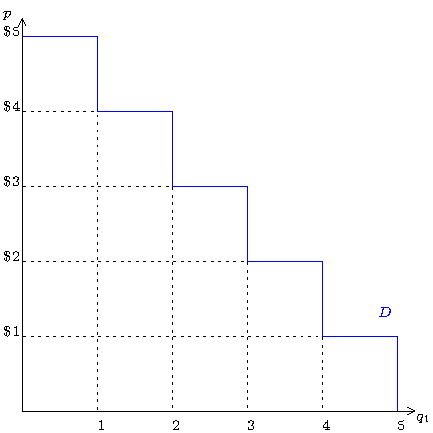
\includegraphics[scale=0.9]{pics/ConsumerWelfare1}
\end{center}
Start with this demand curve: marginal value of first unit is \$5,
second unit is \$4, and so on.
\end{frame}


\begin{frame}
\frametitle{Willingness to pay}
\begin{center}
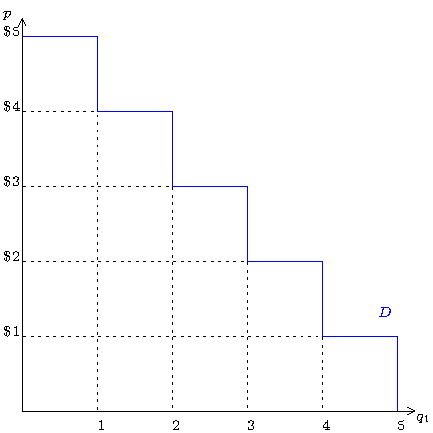
\includegraphics[scale=0.9]{pics/ConsumerWelfare1}
\end{center}
So at price \$5, you buy one unit.\\
At price \$4, you buy two units. And so on.
\end{frame}




\begin{frame}
\frametitle{Willingness to pay}
\begin{center}
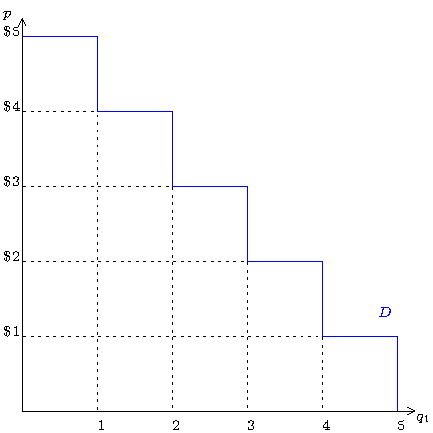
\includegraphics[scale=0.9]{pics/ConsumerWelfare1}
\end{center}
\emph{Consumer surplus}, CS=maximum amount you're willing to pay -
what you pay for it.

\end{frame}




\begin{frame}
\frametitle{Willingness to pay}
\begin{center}
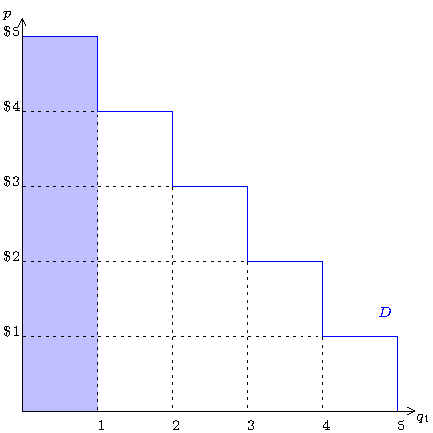
\includegraphics[scale=0.9]{pics/ConsumerWelfare2}
\end{center}
The most you're willing to pay for one unit is the shaded area
(\$$(5\times 1)$).
\end{frame}

\begin{frame}
\frametitle{Willingness to pay}
\begin{center}
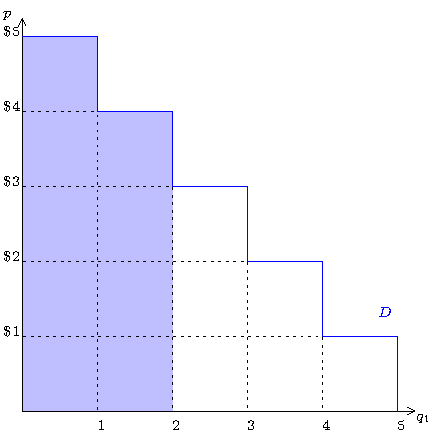
\includegraphics[scale=0.9]{pics/ConsumerWelfare3}
\end{center}
The most you're willing to pay for two units is the shaded area
(\$$(5\times 1) + (4\times 1)$).
\end{frame}


\begin{frame}
\frametitle{Willingness to pay}
\begin{center}
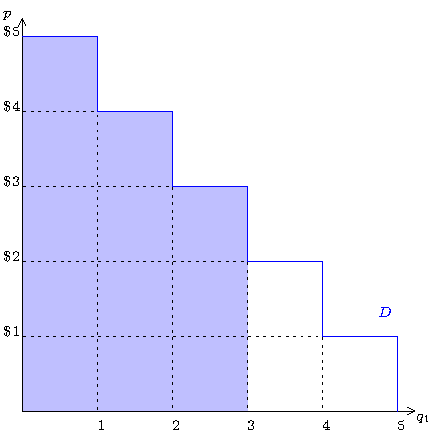
\includegraphics[scale=0.9]{pics/ConsumerWelfare4}
\end{center}
The most you're willing to pay for three units is the shaded area
(\$$(5\times 1) + (4\times 1) + (3\times 1)$).
\end{frame}



\begin{frame}
\frametitle{Calculating consumer surplus}
Suppose that the price is \$3. 
\bigskip

\uncover<2->{ 
You buy three units of the good. 
This costs you  $3\times \$3=\$9.$
}

\end{frame}




\begin{frame}
\frametitle{Calculating consumer surplus}
\begin{center}
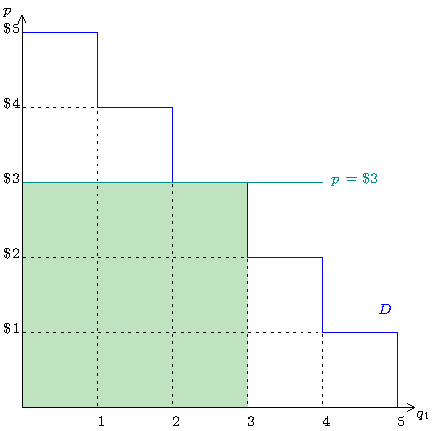
\includegraphics[scale=0.9]{pics/ConsumerWelfare5}
\end{center}
The area of the green shaded area is what you pay for three units if
the price is \$3.

\end{frame}



\begin{frame}
\frametitle{Calculating consumer surplus}
\begin{center}
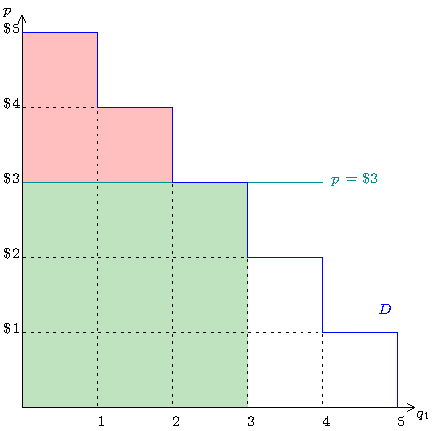
\includegraphics[scale=0.9]{pics/ConsumerWelfare6}
\end{center}
Consumer surplus (red area) = maximum that
you're willing to pay (the previous blue area) - what you paid (the
green area)
\end{frame}




\begin{frame}
\frametitle{Calculating consumer surplus}
CS  consists of three parts:
\bigskip

\uncover<2->{ Surplus from the first unit, $CS_1 = \$5 - \$3=\$2.$}
\bigskip

\uncover<3->{ Surplus from the second unit, $CS_2 = \$4 - \$3=\$1.$}

\bigskip
\uncover<4->{ Surplus from the third unit, $CS_3 = \$3 - \$3=\$0.$}

\uncover<5->{ \[CS= CS_1 + CS_2+CS_3\]}

\end{frame}




\begin{frame}
\frametitle{Consumer surplus}
Equivalent definitions
\begin{enumerate}[<+->]
\item Extra value you get after paying for your desired
amount of a good at a particular price.
\item The most you're willing to pay for the right to buy at a
  particular price.
\item The area under the demand curve and above the price up to the
  quantity demanded at that price.
\end{enumerate}
\end{frame}




\begin{frame}
\frametitle{Consumer surplus of a smooth demand curve}
\begin{center}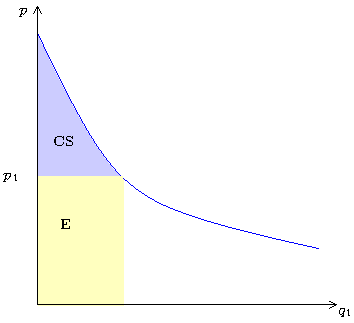
\includegraphics{pics/SmoothConsSurp}\end{center}
CS is the area under the demand curve, above the price.

\bigskip
\uncover<2->{ The area under the demand curve is still the willingness to pay and
you get CS by subtracting expenditure (E).}
\end{frame}




\begin{frame}
\frametitle{Effect of a price change on consumer surplus}
When the price of a good goes up, the consumer is worse off. 

\bigskip
\uncover<2->{ But how much?}
\bigskip

\uncover<3->{ Change in CS is a way to quantify this.}

\end{frame}




\begin{frame}
\frametitle{Effect of a price change on consumer surplus}
\begin{center}
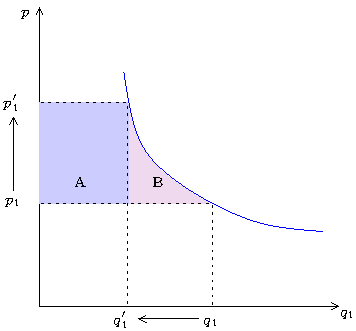
\includegraphics{pics/ChangeInPrice}\end{center}
The change in CS is the sum the areas of regions  A and B.
\bigskip

\uncover<2->{ A is the loss of welfare from paying more for the units you're still
buying.}

\bigskip
\uncover<3->{ B is the loss from buying fewer units.}
\end{frame}

\begin{frame}
\frametitle{Textbook exercise 1.1}

Inverse demand: $p=60-q$.

What is the consumer surplus if the price is 30?
\bigskip

\uncover<2->{
How much is demanded at the price 30? Solve $30=60-q$ for $q$ we find
that $q=30$.
}\bigskip


\uncover<3->{
Let's draw a picture so that we can figure out what CS is.}
\end{frame}

\begin{frame}
\frametitle{Textbook exercise 1.1}
\begin{center}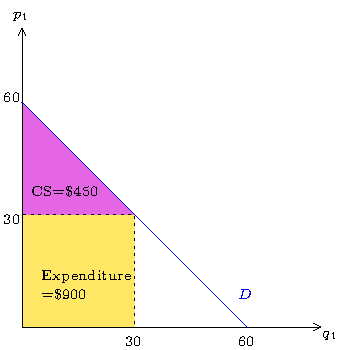
\includegraphics{pics/Exercise1}\end{center}
CS is the area of the pink triangle: base = 30, height = 30.
 \bigskip

CS=Area=$\frac{\text{base}\times\text{height}}{2} = \frac{30\times 30}{2}=450$.
\end{frame}





\begin{frame}
\frametitle{Compensating a consumer for the change in price}
Another way to measure your welfare change:

\uncover<2->{\bigskip
``How much money would I need to give you to keep you as happy as you
were before the price increased?''}

\uncover<3->{\bigskip
We can use the expenditure function to find this.}

\uncover<4->{\bigskip
If your utility was $\overline U$ and the price of good 1 $p_1\to
p_1'$ then }
\uncover<5->{\[
\text{welfare change} = \underset{\text{Costs of getting
    $\overline U$ at $p_1$}}{E(p_1,p_2,\overline U)} -
\underset{\text{Cost of getting
    $\overline U$ at $p_1'$}}{E(p_1',p_2,\overline U)}
\]}
\end{frame}




\begin{frame}
\frametitle{Wich welfare level ($\overline U$) to use?}
Two ways to do it:
\begin{enumerate}[<+->]
\item $\overline U$ is your utility before the price change.
\item $\overline U$ is your utility after the price change.
\end{enumerate}
\end{frame}




\begin{frame}
\frametitle{Compensating variation}
If $\overline U$ is your utility \emph{before} the price change, the
welfare change is the answer to the following question:
\bigskip
\uncover<2->{\begin{center}
``What  would I have to pay you to let me to increase the~price?''
\end{center}}

\uncover<3->{\bigskip
If I give you this amount, you'd be able to buy a bundle
that would keep you at the same utility level $\overline U$ as when
the price doesn't change.}

\uncover<4->{\bigskip
Since I'm \emph{compensating} you for the price increase, we call it
the ``compensating variation'' (CV).}
\end{frame}




\begin{frame}
\frametitle{Equivalent variation}
If $\overline U$ is your utility \emph{after} the price change, the
welfare change is the answer to the following question:
\bigskip
\uncover<2->{\begin{center}
``What would you pay me to stop the price increase?''
\end{center}}
\bigskip
\uncover<3->{If I take away this amount from you but don't change the price, it'll
keep you at the same utility level $\overline U$ as if I change the
price but don't take any money from you.}

\bigskip
\uncover<4->{Since paying me that amount and keeping the prices
and not paying me but having a higher price to give you the same
utility, they're \emph{equivalent}. So we call it the ``equivalent
variation'' (EV).}
\end{frame}




\begin{frame}
\frametitle{An example}
\begin{center}
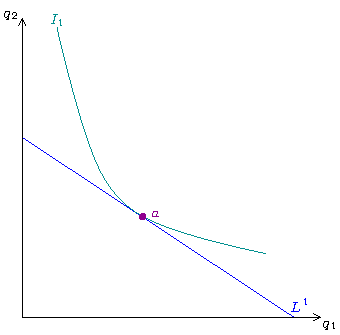
\includegraphics{pics/CVEV}
\end{center}
Suppose that $p_2=1$. We'll see what happens when $p_1$ changes.\\ \
\end{frame}



\begin{frame}
\frametitle{An example}
\begin{center}
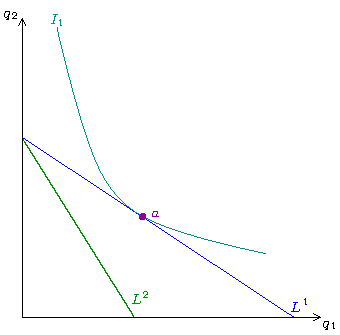
\includegraphics{pics/CVEV1}
\end{center}
When $p_1$ increases, we get the new green budget line.\\ \
\end{frame}




\begin{frame}
\frametitle{An example}
\begin{center}
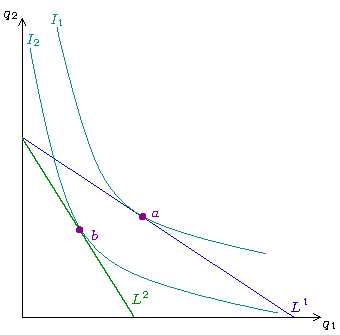
\includegraphics{pics/CVEV2}
\end{center}
From this budget, you pick bundle $b$. You're worse off.\\ \
\end{frame}

\begin{frame}
\frametitle{Compensating variation}
\begin{center}
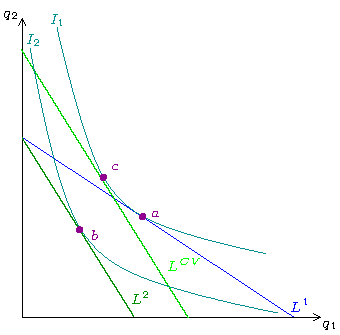
\includegraphics{pics/CVEV3}
\end{center}
If we give you more income at the new price the light green budget
line brings you back to the indifference curve $I^1$.
\end{frame}

\begin{frame}
\frametitle{Compensating variation}
\begin{center}
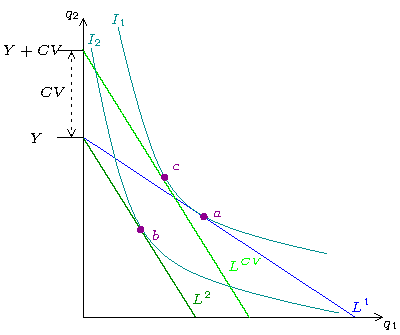
\includegraphics{pics/CVEV4}
\end{center}
If your original income was $Y$, the new income is $Y+CV$.
Since $p_2=1$, this is the vertical distance between the intercepts.\end{frame}



\begin{frame}
\frametitle{Equivalent variation}
\begin{center}
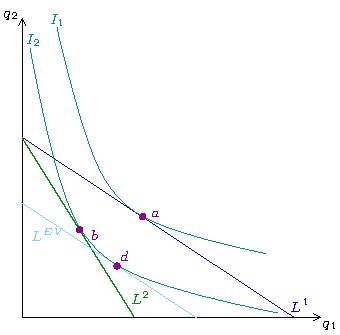
\includegraphics{pics/CVEV5}
\end{center}
If we take away income from you at the old prices, the light blue
budget line brings you to the indifference curve $I^2$.
\end{frame}


\begin{frame}
\frametitle{Equivalent variation}
\begin{center}
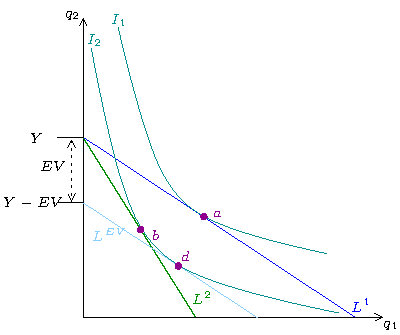
\includegraphics{pics/CVEV6}
\end{center}
If your original income was $Y$, the new income is $Y-EV$.
Since $p_2=1$, this is the vertical distance between the intercepts.
\end{frame}








\begin{frame}
\frametitle{Comparing the three welfare measures}
We've seen three ways of measuring welfare:
\begin{enumerate}
\item Change in consumer surplus ($\Delta$CS)
\item Compensating variation (CV)
\item Equivalent variation (EV)
\end{enumerate}
\bigskip

\uncover<2->{Which one is bigger?
}\bigskip

\uncover<3->{Depends on income elasticity.

Normal goods: $|CV| > |\Delta CS| > |EV|$.

Inferior goods: $|CV| < |\Delta CS| < |EV|$.
}

\uncover<4->{
\bigskip
We can check this graphically. (We'll skip the math:)
}
\end{frame}




\begin{frame}
\frametitle{Comparing the three welfare measures}
\begin{center}
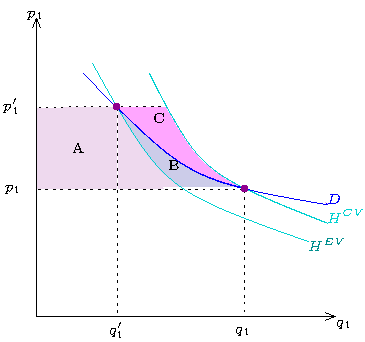
\includegraphics{pics/Compare1}
\end{center}
$|CV| = A+B+C$, $|\Delta CS|=A+B$, and $|EV|=A$.
\bigskip

\uncover<2->{
So $|CV| > |\Delta CS| > |EV|$.}
\bigskip

\end{frame}




\begin{frame}
\frametitle{Comparing the three welfare measures}
Why would this change for an inferior good?
\bigskip

\uncover<2->{The areas B and C are really small compared to A for small changes in
price.}
\bigskip

\uncover<3->{So it often does not matter which measure we use in practice. }
\bigskip

\uncover<4->{Economists usually use CS to measure welfare since it's easy to
calculate from the observable demand function.}
\end{frame}




\begin{frame}
\frametitle{Market consumer surplus}
Recall: You get market demand by horizontally adding up individual
demand.

\bigskip
\uncover<2->{The effect of a price increase on CS is calculated the same way for
the market as a whole as it is for individuals.}
\end{frame}






\begin{frame}
\frametitle{Market consumer surplus}
\begin{center}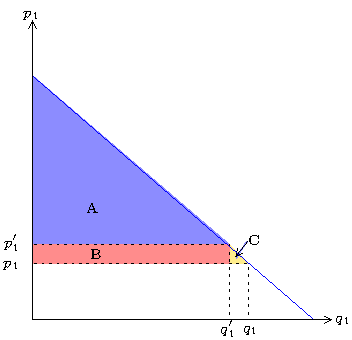
\includegraphics{pics/MarketCS}
\end{center}
\uncover<2->{CS before price increase: A+B+C\\}
\uncover<3->{CS after price increase: A\\}
\uncover<4->{Loss of CS because of price increase: B+C}
\end{frame}




\begin{frame}
\frametitle{Markets in which CS Loss is large}
CS is loss is bigger 
\begin{enumerate}[<+->]
\item The more money is spent on the good (revenue from sales of
  the good), $pQ$: This makes A, B, and C all bigger. \\ \
\item The less elastic demand is: B is bigger as demand gets more
  inelastic. This is because consumers buy a similar quantity even as
  the price rises.
\end{enumerate}
\end{frame}

\begin{frame}
\frametitle{Textbook exercise  3.4}
Two linear demand curves go through the initial equilibrium $e_1$. One
demand curve is less elastic   than the other at $e_1$. For which
demand curve will a price increase cause the larger consumer surplus
loss?
\bigskip

\uncover<2->{Since they both pass through the same point $e_1$, the
  less elastic demand curve is steeper than the more elastic
  one. That's because $\frac{dQ}{dp}$ is larger in absolute value for
  the more elastic one.
}
\end{frame}

\begin{frame}
\frametitle{Textbook exercise 3.4}
\begin{center}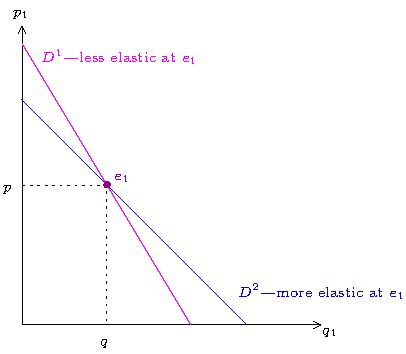
\includegraphics{pics/Exercise3}\end{center}
\bigskip

\
\end{frame}
\begin{frame}
\frametitle{Textbook exercise 3.4}
\begin{center}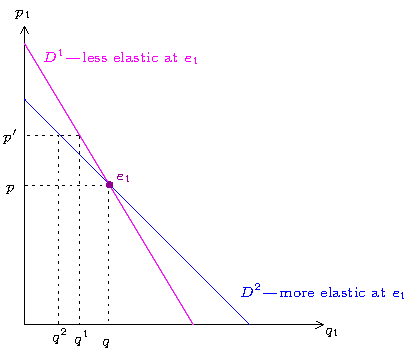
\includegraphics{pics/Exercise31}\end{center}
If price increase to $p'$, quantities change to $q^1$ and $q^2$.
\end{frame}


\begin{frame}
\frametitle{Textbook exercise 3.4}
\begin{center}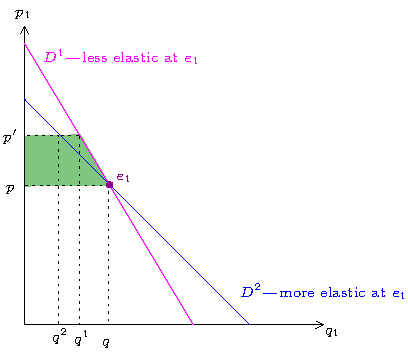
\includegraphics{pics/Exercise32}\end{center}
The green shaded area is the loss of CS for $D^1$
\end{frame}



\begin{frame}
\frametitle{Textbook exercise 3.4}
\begin{center}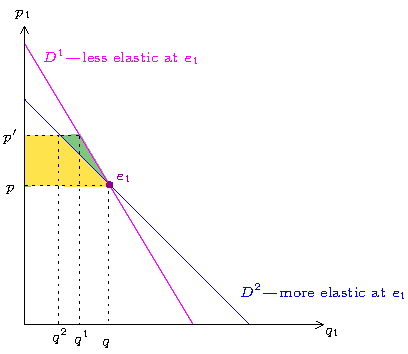
\includegraphics{pics/Exercise33}\end{center}
The yellow shaded area is the loss of CS for $D^2$. 
\end{frame}






\begin{frame}
\frametitle{Effects of government policies on consumer welfare}
We'll look at two kinds of policies:
\begin{enumerate}[<+->]
\item Quotas: a limit on the amount of a good a person can
  purchase. 
\item Subsidies on the price of a good.
\end{enumerate}
\end{frame}




\begin{frame}
\frametitle{Quotas}
\begin{center}
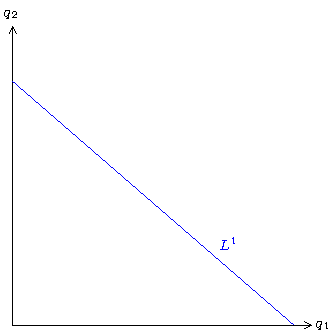
\includegraphics{pics/Quota1}
\end{center}
You start with this budget set (both prices are \$1).
\end{frame}


\begin{frame}
\frametitle{Quotas}
\begin{center}
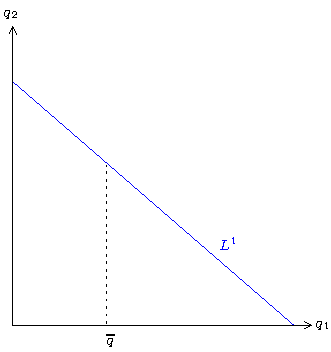
\includegraphics{pics/Quota2}
\end{center}
Suppose you have a quota of $\overline q$.
\end{frame}




\begin{frame}
\frametitle{Quotas}
\begin{center}
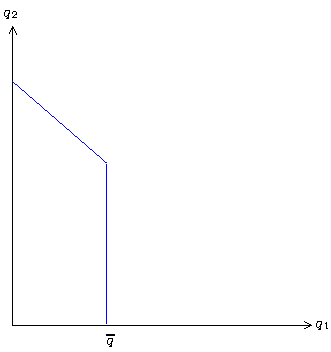
\includegraphics{pics/Quota3}
\end{center}
Now, you can only select from this set.
\end{frame}

\begin{frame}
\frametitle{Quotas}
\begin{center}
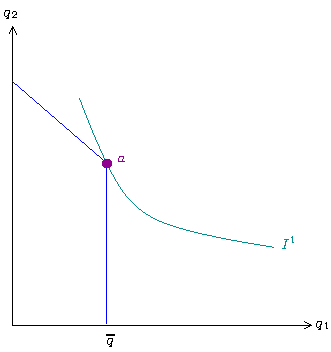
\includegraphics{pics/Quota4}
\end{center}
You pick your favorite bundle.
\end{frame}


\begin{frame}
\frametitle{Quotas}
\begin{center}
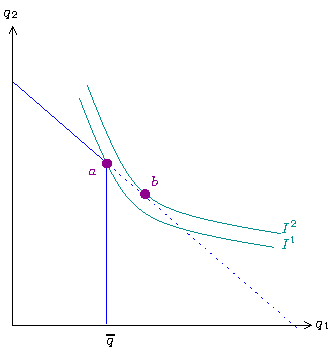
\includegraphics{pics/Quota5}
\end{center}
You're worse off than without the quota.
\end{frame}


\begin{frame}
\frametitle{Quotas}
\begin{center}
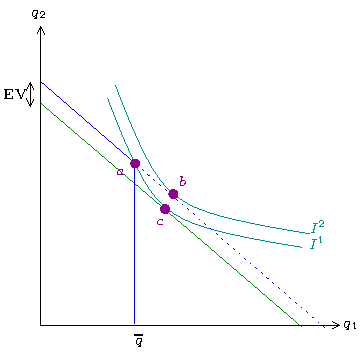
\includegraphics{pics/Quota6}
\end{center}
It's as though your income was reduced by EV.
\end{frame}




\begin{frame}
\frametitle{Subsidized goods}
Many subsidies are such that the consumer is given a certain amount of
a good at no charge. 
\bigskip

\uncover<2->{The consumer only pays for any of the good that he buys above that
amount.}

\bigskip
\uncover<3->{Examples: daycare in Canada, food stamps in the US.}

\end{frame}


\begin{frame}
\frametitle{Subsidized goods}
\begin{center}
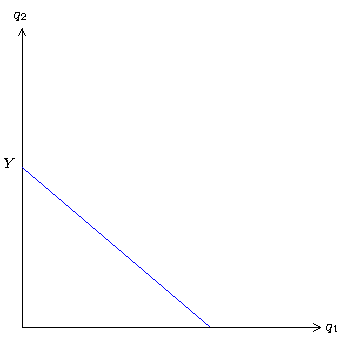
\includegraphics{pics/Subsidy1}
\end{center}
Without a subsidy this is your budget line (both prices are \$1). 
\end{frame}


\begin{frame}
\frametitle{Subsidized goods}
\begin{center}
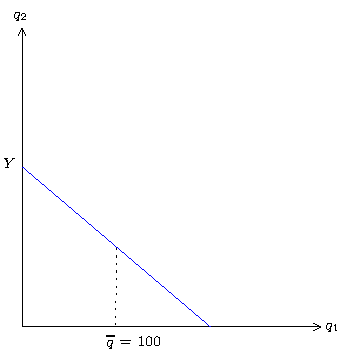
\includegraphics{pics/Subsidy2}
\end{center}
Suppose the first $\overline q$ units are free.
\end{frame}


\begin{frame}
\frametitle{Subsidized goods}
\begin{center}
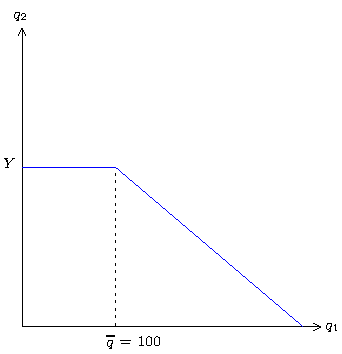
\includegraphics{pics/Subsidy3}
\end{center}
Your now pick from this set.
\end{frame}


\begin{frame}
\frametitle{Subsidized goods}
\begin{center}
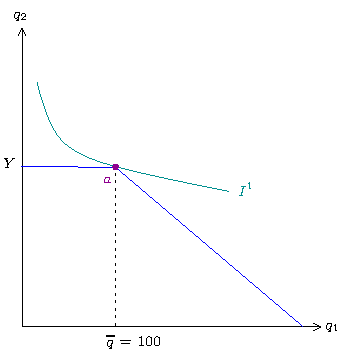
\includegraphics{pics/Subsidy4}
\end{center}
You might choose bundle $a$.
\end{frame}


\begin{frame}
\frametitle{Subsidized goods}
\begin{center}
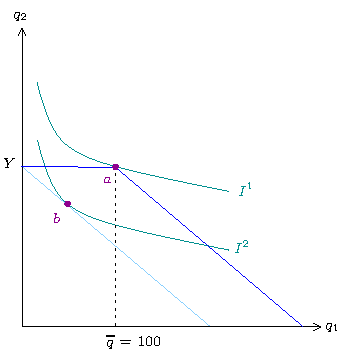
\includegraphics{pics/Subsidy5}
\end{center}
You're better off than without the subsidy when you'd choose b.
\end{frame}

\begin{frame}
\frametitle{Subsidized goods}
\begin{center}
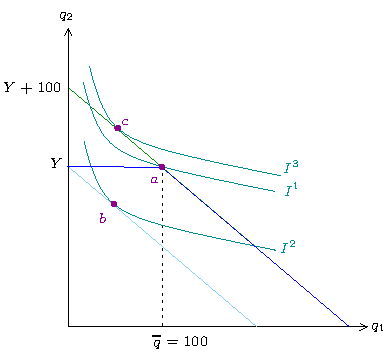
\includegraphics{pics/Subsidy6}
\end{center}
You'd be prefer \$100 in cash to 100 free units of good 1.
\end{frame}

\begin{frame}
\frametitle{Subsidized goods}
\begin{center}
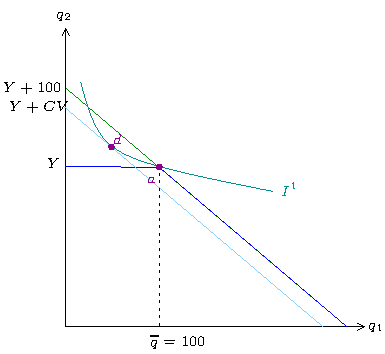
\includegraphics{pics/Subsidy7}
\end{center}
You'd be just as happy with \$CV in cash as with the subsidy.
\end{frame}

\begin{frame}
\frametitle{Subsidized goods}
\begin{center}
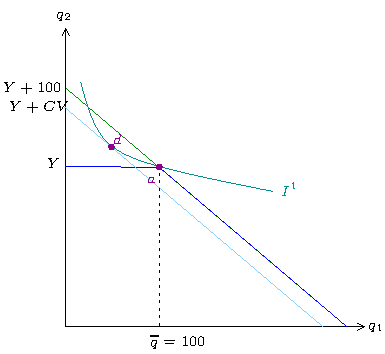
\includegraphics{pics/Subsidy7}
\end{center}
If we took away the subsidy, we'd have to give you $\$CV$ to
compensate you.
\end{frame}



\begin{frame}
\frametitle{A word of caution}
The exercise of quantifying the losses from these kinds of policies
should not be interpreted as saying that there should never be such
policies.
\bigskip

\uncover<2->{This is a way of measuring the cost of the policies. When making
decisions, these costs must be weighed against benefits from the
intended  goals of the policies.}
\end{frame}



\end{document}






